\documentclass{article}

% if you need to pass options to natbib, use, e.g.:
% \PassOptionsToPackage{numbers, compress}{natbib}
% before loading nips_2018

% ready for submission
%\usepackage{nips_2018}

% to compile a preprint version, e.g., for submission to arXiv, add
% add the [preprint] option:
\usepackage[preprint]{nips_2018}

% to compile a camera-ready version, add the [final] option, e.g.:
% \usepackage[final]{nips_2018}

% to avoid loading the natbib package, add option nonatbib:
% \usepackage[nonatbib]{nips_2018}

\usepackage[utf8]{inputenc} % allow utf-8 input
\usepackage[T1]{fontenc}    % use 8-bit T1 fonts
\usepackage{hyperref}       % hyperlinks
\usepackage{url}            % simple URL typesetting
\usepackage{booktabs}       % professional-quality tables
\usepackage{amsfonts}       % blackboard math symbols
\usepackage{nicefrac}       % compact symbols for 1/2, etc.
\usepackage{microtype}      % microtypography
\usepackage{graphicx}       % include graphics

\title{Multiple Track MIDI Generation}

% The \author macro works with any number of authors. There are two
% commands used to separate the names and addresses of multiple
% authors: \And and \AND.
%
% Using \And between authors leaves it to LaTeX to determine where to
% break the lines. Using \AND forces a line break at that point. So,
% if LaTeX puts 3 of 4 authors names on the first line, and the last
% on the second line, try using \AND instead of \And before the third
% author name.

\author{
  Bryan Learn\\
  10-701\\
  Carnegie Mellon University\\
  Pittsburgh, PA 15213\\
  \And
  Mike Tasota\\
  10-701\\
  Carnegie Mellon University\\
  Pittsburgh, PA 15213\\
}

\begin{document}
% \nipsfinalcopy is no longer used

\maketitle


\section{Introduction}

Although similar to text generation in many respects, there is still significant progress to be made in the area of music generation. There are a few distinctions between the problem of music generation and text generation that affect this. The number of potential states that a standard 88-key piano can take greatly exceeds the number of words in any language. Another difference that is present in music generation is the concept of tempo, which adds even more complexity to the number of representations that generated music can take in comparison to generated text.

Previous rule-based models of generation are now being outperformed thanks to the advent of deep learning techniques. One research effort that has made significant progress is the Magenta research project, which was started by researchers and engineers from the Google Brain team. This package utilizes the TensorFlow library to implement various deep learning techniques for the problem of music generation.


\section{Related Work}
In the MidiNet paper, Yang et al. created a CNN-GAN based model for MIDI generation. They propose that their model could be possibly expanded to generate multiple tracks. This was demonstrated in the work done by MuseGAN. However, as pointed out in the MusicVAE paper, MuseGAN works with a fixed set of instruments, namely bass, drums, guitar, piano, and strings. Instead, MusicVAE is capable of modeling exactly three broad classes of instruments which it calls the “trio:” melody, bass, and drums. This provides more flexibility on what instruments can be assigned in track generation. However, it also introduces chord conditioning to keep harmony fixed.

Another related work in multiple track generation is from Chu et al. in their “Song from PI” RNN. Although PI is capable of producing multiple tracks, they also conditioned the generation on scale types to help pick up regularities in their dataset of pop songs. In our work, we hope to produce multiple tracks without relying on prior knowledge of music theory in the model.


\section{Proposed Work}
We will explore the possibilities of creating music generation models that can learn specific types of instrument classes without being explicitly defined. As we plan to do this within the Magenta project framework, the representation used to train and generate musical content will be MIDI files with single and multiple tracks. Furthermore, we will leave it as a task for the models to learn the underlying chord structures instead of explicitly conditioning the generation on music theory concepts. We will compare models based on both a Recurrent Neural Network (RNN) and a Variational Autoencoder (VAE) to see if there are any significant differences in performance on this task. Since generating melody has already been targeted in previous work, examples of other instrument classes to train on may include: drums, bass, and chords.

After focusing on generation of a second track, if time permits, we will expand our work to a third track which can then be generalized to any number of tracks. Another important thing to consider is the interdependence of tracks. As discussed in ``Song from PI'', one approach is to assume that tracks are independent given a melody. An alternative approach is to learn a third track given a second track and a melody. Again, we would like to explore all options to compare results.


\section{Preliminary Results}

As an initial evaluation of music complexity and aesthetic from the related works, small batches of samples were generated from three different models. We compared pre-trained models released by Google Magenta: MeldoyRNN \verb|basic_rnn|, MusicVAE \verb|mel_16bar|, and MusicVAE \verb|trio_16bar|. We evaluated the generated samples by comparing the visual representations and listening to the samples.

\begin{figure}[htb!]
  \begin{minipage}{0.48\textwidth}
    \centering
    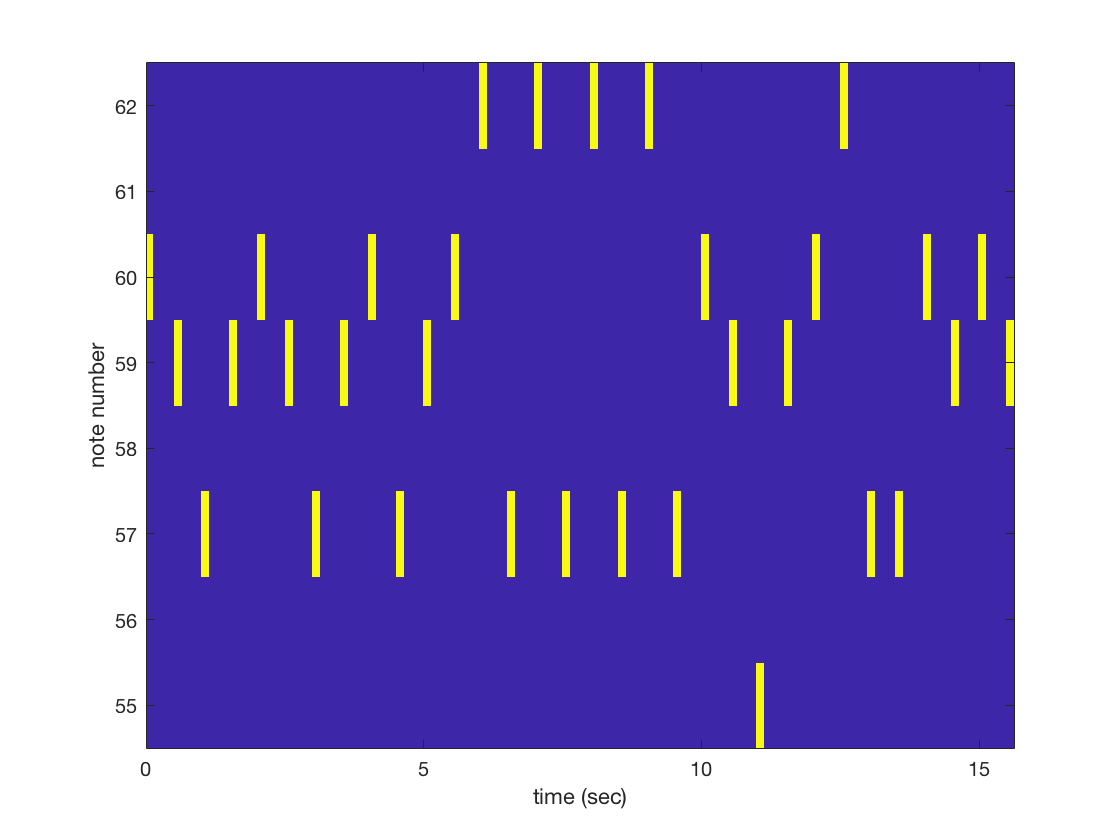
\includegraphics[height=4cm, width=4cm]{melody_rnn.png}
    \caption{MelodyRNN: basic RNN model.}
  \end{minipage}
  \begin{minipage}{0.48\textwidth}
    \centering
    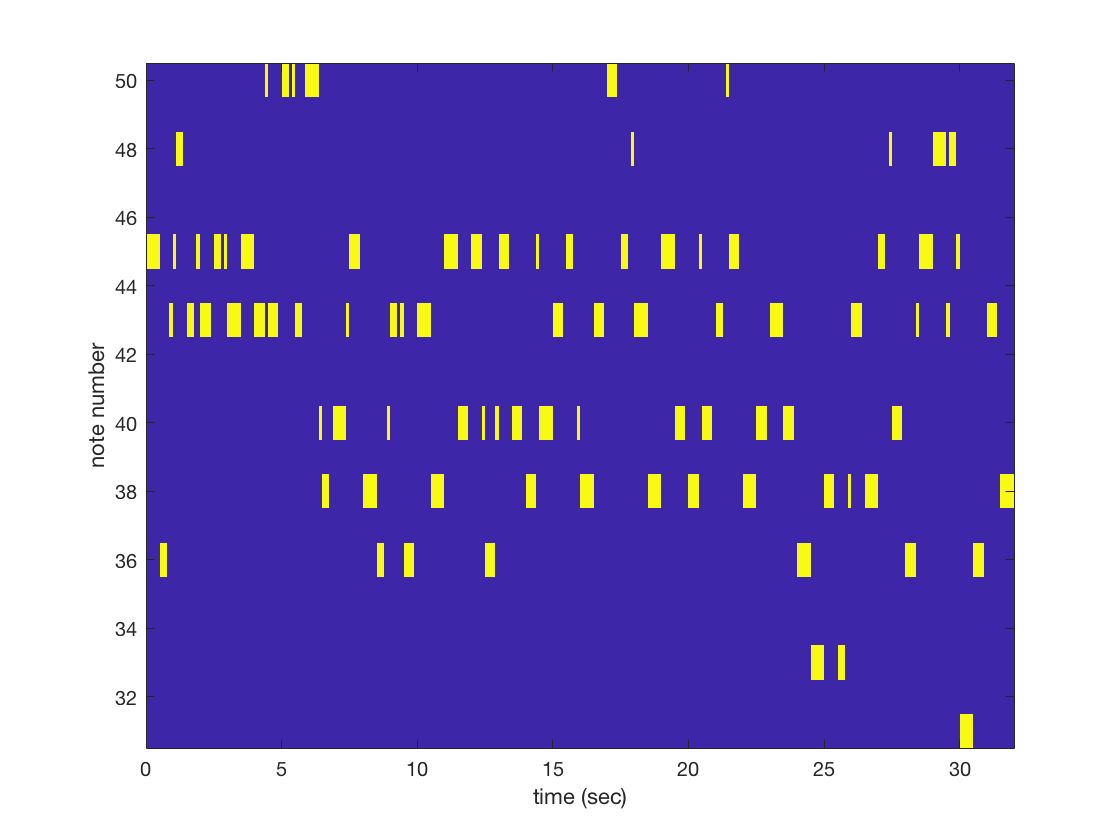
\includegraphics[height=4cm, width=4cm]{musicvae_melody.png}
    \caption{MusicVAE: hierarchical melody model.}
  \end{minipage}\hfill
  \begin{minipage}{0.48\textwidth}
    \centering
    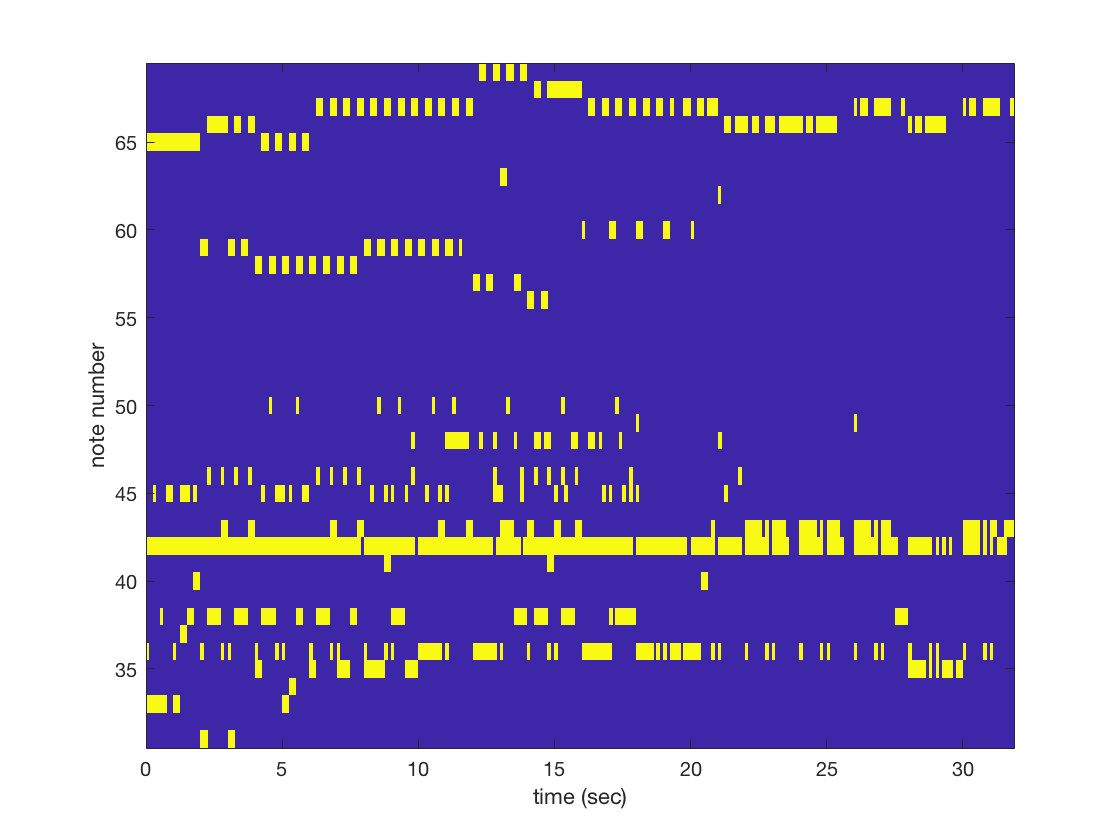
\includegraphics[height=4cm, width=4cm]{musicvae_trio.png}
    \caption{MusicVAE: hierarchical trio model.}
  \end{minipage}
\end{figure}

The most complex samples came from the MusicVAE trio model although it relies on chord conditioning while the others do not. This was the only model that generates multiple tracks. It will be interesting to see if we can generate sequence that are comparably complex without chord conditioning. The samples generated from the MelodyRNN model were more simplistic compared to the output of both MusicVAE models. It is still to be determined if this will be the case when multiple tracks are generated.

\section*{References}

\small

[1] Chu, Hang, et al. ``Song From PI: A Musically Plausible Network for Pop Music Generation.'' {\it [1611.03477] Song From PI: A Musically Plausible Network for Pop Music Generation,} 10 Nov. 2016, arxiv.org/abs/1611.03477.

[2] Simon, Ian, et al. ``Learning a Latent Space of Multitrack Measures.'' {\it[1806.00195] Learning a Latent Space of Multitrack Measures,} 1 June 2018, arxiv.org/abs/1806.00195.

[3] Yang, Li-Chia, et al. ``MidiNet: A Convolutional Generative Adversarial Network for Symbolic-Domain Music Generation.'' {\it[1703.10847] MidiNet: A Convolutional Generative Adversarial Network for Symbolic-Domain Music Generation,} 18 July 2017, arxiv.org/abs/1703.10847.

\end{document}